\chapter{De mol en de molaire massa}\label{ch:g10:the-mole}

Aan het eind van de dag telt een bank haar munten niet een voor een: ze
weegt ze. Als één munt een massa van \qty{7.5}{g} heeft, bevat een zak
munten met een massa van \qty{7.5}{kg} duizend munten, en de weegschaal
heeft het tellen gedaan. Scheikundigen hebben hetzelfde probleem met
\omterm{def:g7:atoms-and-molecules:atom}{atomen}, alleen veel erger: een lepel water bevat meer \omterm{def:g7:atoms-and-molecules:molecule}{moleculen} dan er
zandkorrels liggen op alle stranden van een hele kust. Ze lossen het op
dezelfde manier op, door te wegen, en de zak die ze gebruiken bevat
\num{602214076000000000000000} deeltjes. Dit hoofdstuk definieert die
zak, de \omterm{def:g10:the-mole:amount}{mol}, en laat zien hoe je van een massa op een balans naar een
aantal \omterm{def:g7:atoms-and-molecules:atom}{atomen} of \omterm{def:g7:atoms-and-molecules:molecule}{moleculen} gaat.

\begin{recall}
De massa van een \omterm{def:g7:atoms-and-molecules:atom}{atoom} zit geconcentreerd in zijn kern; een \omterm{def:g9:inside-the-atom:proton}{proton} en een
\omterm{def:g9:inside-the-atom:proton}{neutron} hebben elk een massa van ongeveer \qty{1.67e-27}{kg}, dus een
\omterm{def:g7:atoms-and-molecules:atom}{atoom} met \omterm{def:g9:inside-the-atom:atomic-number}{massagetal} $A$ heeft een massa van ongeveer
$A \times \qty{1.67e-27}{kg}$. Heel grote en heel kleine getallen schrijf
je in wetenschappelijke notatie (\cref{ch:g9:inside-the-atom}). Een
\omterm{def:g7:atoms-and-molecules:formula}{chemische formule} geeft het aantal \omterm{def:g7:atoms-and-molecules:atom}{atomen} van elk element in een \omterm{def:g7:atoms-and-molecules:molecule}{molecuul}
(\cref{ch:g7:atoms-and-molecules}).
\end{recall}

\begin{omfigure}
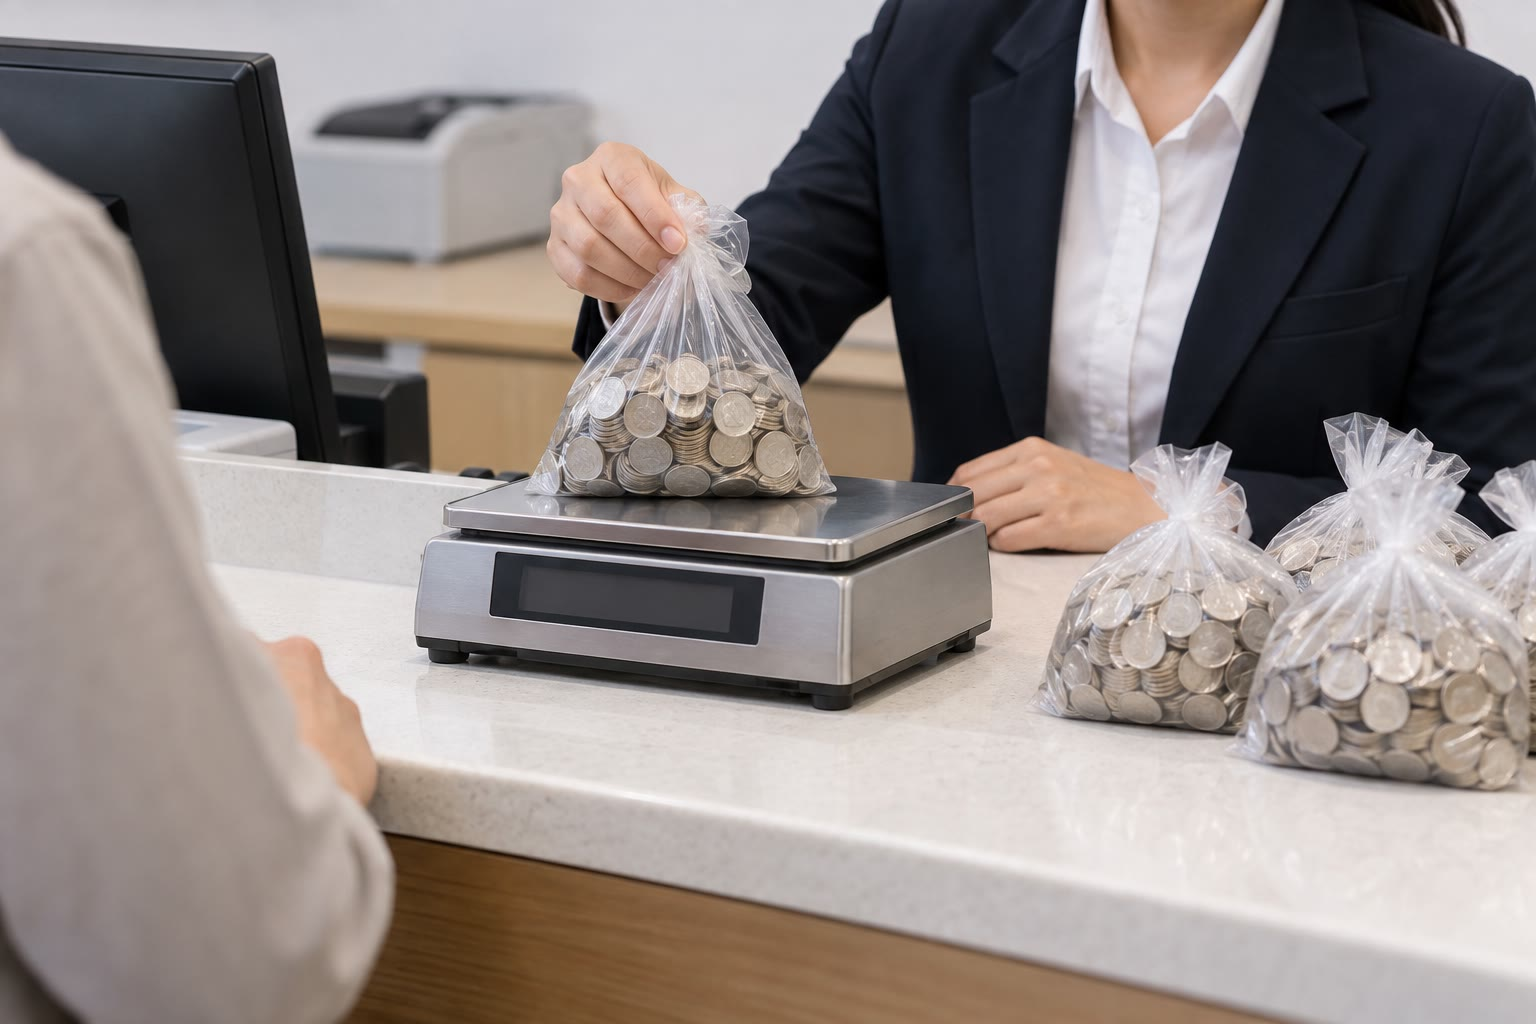
\includegraphics[width=0.55\linewidth]{images/book1/ai/g10-bank-coins.jpg}

{\small Een bank telt munten door ze te wegen. Scheikundigen tellen
\omterm{def:g7:atoms-and-molecules:atom}{atomen} op dezelfde manier.}
\end{omfigure}

\section{Tellen door te wegen}

\begin{example}[Een zak munten]\label{ex:g10:the-mole:coins}
Een munt heeft een massa van \qty{7.5}{g}. Een zak met zulke munten heeft
een massa van \qty{1.80}{kg}, dat is \qty{1800}{g}, zonder de zak zelf
mee te tellen. Hij bevat
\[
  \frac{\qty{1800}{g}}{\qty{7.5}{g}} = 240 \text{ munten.}
\]
Om te tellen, deelt de bank de totale massa door de massa van één munt.
\end{example}

\begin{example}[Een lepel water]\label{ex:g10:the-mole:spoon}
Een watermolecuul, \ce{H2O}, heeft $2 + 16 = 18$ \omterm{def:g9:inside-the-atom:proton}{nucleonen} (\omterm{def:g7:atoms-and-molecules:atom}{atomen}
zuurstof-16 en waterstof-1 vormen bijna al het natuurlijke water), dus
zijn massa is ongeveer $18 \times \qty{1.67e-27}{kg} = \qty{3.0e-26}{kg}$,
of \qty{3.0e-23}{g}. Een lepel met \qty{5.0}{g} water bevat dus
\[
  \frac{\qty{5.0}{g}}{\qty{3.0e-23}{g}} \approx \num{1.7e23}
  \text{ moleculen.}
\]
De deling werkt zoals bij de munten, maar de uitkomst is een getal dat
niemand zich kan voorstellen. Scheikundigen hebben een pakket \omterm{def:g7:atoms-and-molecules:atom}{atomen}
nodig dat past bij de monsters in het laboratorium.
\end{example}

\begin{definition}[Hoeveelheid stof en mol]\label{def:g10:the-mole:amount}
% ledger: const:NA
De \emph{hoeveelheid stof}\index{hoeveelheid stof} $n$ van een monster
telt de deeltjes die het bevat (\omterm{def:g7:atoms-and-molecules:atom}{atomen}, \omterm{def:g7:atoms-and-molecules:molecule}{moleculen} of \omterm{def:g9:ions:ion}{ionen}, telkens te
vermelden). De eenheid is de \emph{mol}\index{mol}, symbool \si{mol}: één
mol bevat precies \num{6.02214076e23} deeltjes.
\end{definition}

\begin{remark}[Een dozijn, een riem, een mol]\label{rem:g10:the-mole:dozen}
De \omterm{def:g10:the-mole:amount}{mol} is een telwoord, zoals een dozijn eieren (12) of een riem papier
(500 vellen), alleen veel groter. ``Twee \omterm{def:g10:the-mole:amount}{mol} watermoleculen'' betekent
$2 \times \num{6.02214076e23} = \num{1.20e24}$ \omterm{def:g7:atoms-and-molecules:molecule}{moleculen}, zoals ``twee
dozijn eieren'' 24 eieren betekent. Zeg altijd welke deeltjes je telt:
één \omterm{def:g10:the-mole:amount}{mol} zuurstof\emph{\omterm{def:g7:atoms-and-molecules:molecule}{moleculen}} \ce{O2} bevat twee \omterm{def:g10:the-mole:amount}{mol}
zuurstof\emph{\omterm{def:g7:atoms-and-molecules:atom}{atomen}}.
\end{remark}

\begin{history}[De hypothese van Avogadro, 1811]
In 1811 stelde de natuurkundige Amedeo Avogadro voor dat gelijke volumes
van verschillende gassen, bij dezelfde temperatuur en druk, evenveel
deeltjes bevatten. Hij begreep ook dat een gas als zuurstof bestaat uit
\omterm{def:g7:atoms-and-molecules:molecule}{moleculen} van twee \omterm{def:g7:atoms-and-molecules:atom}{atomen}. Zijn idee werd bijna vijftig jaar genegeerd,
tot Stanislao Cannizzaro het in 1860 gebruikte om een samenhangende reeks
atoomgewichten te verkrijgen. De constante die de deeltjes in een \omterm{def:g10:the-mole:amount}{mol}
telt, werd later naar Avogadro genoemd; hij heeft de waarde nooit
gekend.
\end{history}

\begin{omfigure}
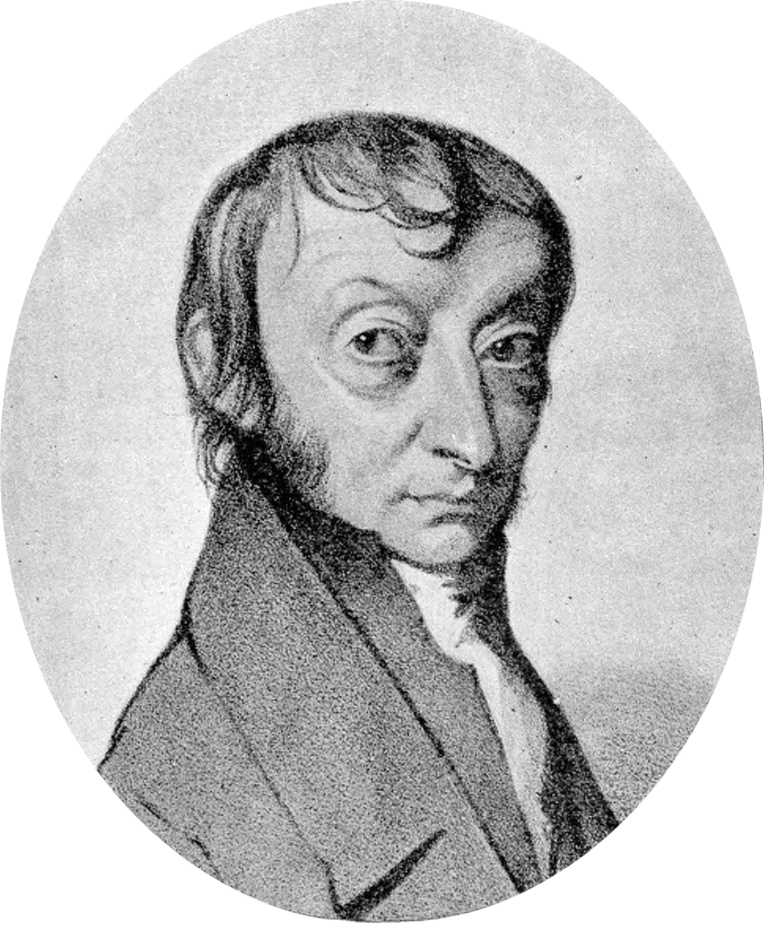
\includegraphics[width=0.26\linewidth]{images/book1/avogadro.jpg}

{\small Amedeo Avogadro (1776--1856).}
\end{omfigure}

\section{De constante van Avogadro}

\begin{definition}[Constante van Avogadro]\label{def:g10:the-mole:avogadro}
% ledger: const:NA
De \emph{constante van Avogadro}\index{constante van Avogadro} $N_A$ is
het aantal deeltjes per \omterm{def:g10:the-mole:amount}{mol}:
\[
  N_A = \qty{6.02214076e23}{mol^{-1}} .
\]
De waarde is exact, vastgelegd door de definitie. In berekeningen rond je
haar af op \qty{6.02e23}{mol^{-1}}.
\end{definition}

\begin{proposition}[Aantal deeltjes en hoeveelheid stof]\label{prop:g10:the-mole:number}
Een monster met $N$ deeltjes bevat de \omterm{def:g10:the-mole:amount}{hoeveelheid stof}
\[
  n = \frac{N}{N_A}, \qquad\text{dus}\qquad N = n \times N_A .
\]
\end{proposition}

\begin{proof}
Elke \omterm{def:g10:the-mole:amount}{mol} bevat $N_A$ deeltjes, dus $n$ \omterm{def:g10:the-mole:amount}{mol} bevat $n \times N_A$
deeltjes; delen door $N_A$ geeft $n$.
\end{proof}

\begin{example}[Moleculen en mol]\label{ex:g10:the-mole:convert}
Een monster bevat \num{1.5e24} \omterm{def:g7:atoms-and-molecules:molecule}{moleculen} koolstofdioxide. De hoeveelheid
koolstofdioxide is
$n = \num{1.5e24} / \qty{6.02e23}{mol^{-1}} = \qty{2.5}{mol}$.
Omgekeerd bevat \qty{0.20}{mol} ijzer
$N = \qty{0.20}{mol} \times \qty{6.02e23}{mol^{-1}} = \num{1.2e23}$
ijzeratomen.
\end{example}

\begin{remark}[Waar het getal vandaan komt]\label{rem:g10:the-mole:origin}
Meer dan vijftig jaar lang was de \omterm{def:g10:the-mole:amount}{mol} gedefinieerd als het aantal \omterm{def:g7:atoms-and-molecules:atom}{atomen}
in precies \qty{12}{g} koolstof-12, en moest $N_A$ gemeten worden. Sinds
2019 ligt het getal zelf vast, waardoor de \omterm{def:g10:the-mole:amount}{mol} een zuivere telling is.
De oude en de nieuwe definitie komen overeen tot op minder dan één deel
op honderd miljoen, dus twaalf gram koolstof-12 bevat nog steeds één \omterm{def:g10:the-mole:amount}{mol}
\omterm{def:g7:atoms-and-molecules:atom}{atomen}, zoals de volgende paragraaf controleert.
\end{remark}

\section{Molaire massa}

\begin{definition}[Molaire massa]\label{def:g10:the-mole:molar-mass}
De \emph{molaire massa}\index{molaire massa} $M$ van een \omterm{def:g6:pure-substances-and-mixtures:species}{chemische stof}
is de massa van één \omterm{def:g10:the-mole:amount}{mol} van haar deeltjes, in gram per \omterm{def:g10:the-mole:amount}{mol}
(\si{g/mol}). De molaire massa van een element, genomen over zijn
natuurlijke \omterm{def:g6:pure-substances-and-mixtures:mixture}{mengsel} van \omterm{def:g9:inside-the-atom:isotope}{isotopen}, is zijn \emph{molaire
atoommassa}\index{molaire atoommassa}; die staat in het \omterm{def:g9:periodic-table-first-look:periodic-table}{periodiek
systeem}.
\end{definition}

\begin{example}[Eén mol koolstofatomen]\label{ex:g10:the-mole:carbon}
% ledger: const:NA, const:u
Een \omterm{def:g7:atoms-and-molecules:atom}{atoom} koolstof-12 heeft een massa van ongeveer
$12 \times \qty{1.67e-27}{kg} = \qty{2.00e-26}{kg}$. Eén \omterm{def:g10:the-mole:amount}{mol} ervan
heeft een massa van
\[
  \qty{2.00e-26}{kg} \times \num{6.02e23} = \qty{1.20e-2}{kg}
  = \qty{12.0}{g}.
\]
De \omterm{def:g10:the-mole:amount}{mol} is zo gekozen dat de \omterm{def:g10:the-mole:molar-mass}{molaire massa} van een \omterm{def:g7:atoms-and-molecules:atom}{atoom}, in gram per \omterm{def:g10:the-mole:amount}{mol},
dicht bij zijn \omterm{def:g9:inside-the-atom:atomic-number}{massagetal} ligt: ongeveer \qty{1}{g/mol} voor waterstof,
\qty{12}{g/mol} voor koolstof, \qty{16}{g/mol} voor zuurstof.
\end{example}

\begin{omfigure}
% ledger: aw:H, aw:C, aw:N, aw:O, aw:Na, aw:Mg, aw:Al, aw:Si, aw:S, aw:Cl, aw:K, aw:Ca, aw:Fe, aw:Cu, aw:Zn, aw:Au (rounded to 0.1)
\begin{tabular}{lcr@{\qquad}lcr}
\hline
element & symbool & $M$ (\si{g/mol}) & element & symbool & $M$ (\si{g/mol}) \\
\hline
waterstof & \ce{H}  & 1.0  & silicium  & \ce{Si} & 28.1 \\
koolstof  & \ce{C}  & 12.0 & zwavel    & \ce{S}  & 32.1 \\
stikstof  & \ce{N}  & 14.0 & chloor    & \ce{Cl} & 35.5 \\
zuurstof  & \ce{O}  & 16.0 & kalium    & \ce{K}  & 39.1 \\
natrium   & \ce{Na} & 23.0 & calcium   & \ce{Ca} & 40.1 \\
magnesium & \ce{Mg} & 24.3 & ijzer     & \ce{Fe} & 55.8 \\
aluminium & \ce{Al} & 27.0 & koper     & \ce{Cu} & 63.5 \\
          &         &      & goud      & \ce{Au} & 197.0 \\
\hline
\end{tabular}\par\medskip

{\small \omterm{def:g10:the-mole:molar-mass}{Molaire atoommassa}'s van veelvoorkomende elementen, afgerond op
\qty{0.1}{g/mol}. Dit zijn de waarden die in dit boek gebruikt worden.}
\end{omfigure}

\begin{remark}[Waarom chloor 35.5 is]\label{rem:g10:the-mole:chlorine}
% ledger: iso:Cl35, iso:Cl37
Natuurlijk chloor is een \omterm{def:g6:pure-substances-and-mixtures:mixture}{mengsel} van twee \omterm{def:g9:inside-the-atom:isotope}{isotopen}: ongeveer drie kwart
van de \omterm{def:g7:atoms-and-molecules:atom}{atomen} is chloor-35, een kwart chloor-37
(\cref{ch:g9:inside-the-atom}). De \omterm{def:g10:the-mole:molar-mass}{molaire atoommassa} is het gemiddelde,
gewogen met deze aandelen, en ligt tussen 35 en 37: \qty{35.5}{g/mol}.
Daarom liggen sommige \omterm{def:g10:the-mole:molar-mass}{molaire atoommassa}'s ver van gehele getallen.
\end{remark}

\begin{proposition}[Molaire massa van een molecuul]\label{prop:g10:the-mole:sum}
De \omterm{def:g10:the-mole:molar-mass}{molaire massa} van een \omterm{def:g7:atoms-and-molecules:molecule}{molecuul} is de som van de \omterm{def:g10:the-mole:molar-mass}{molaire atoommassa}'s
van al zijn \omterm{def:g7:atoms-and-molecules:atom}{atomen}, elk zo vaak geteld als het in de formule voorkomt.
Met dezelfde regel bereken je de \omterm{def:g10:the-mole:molar-mass}{molaire massa} van een ionaire vaste stof
uit haar formule-eenheid.
\end{proposition}

\begin{proof}
Eén \omterm{def:g10:the-mole:amount}{mol} \omterm{def:g7:atoms-and-molecules:molecule}{moleculen} \ce{A_xB_y} bevat $x$ \omterm{def:g10:the-mole:amount}{mol} \omterm{def:g7:atoms-and-molecules:atom}{atomen} \ce{A} en $y$ \omterm{def:g10:the-mole:amount}{mol}
\omterm{def:g7:atoms-and-molecules:atom}{atomen} \ce{B}, en verder niets; de massa is de som van hun massa's,
$x\,M(\ce{A}) + y\,M(\ce{B})$.
\end{proof}

\begin{example}[Drie molaire massa's]\label{ex:g10:the-mole:three}
% ledger: aw:H, aw:C, aw:O, aw:Na, aw:Cl
\begin{align*}
  M(\ce{H2O}) &= 2 \times 1.0 + 16.0 = \qty{18.0}{g/mol},\\
  M(\ce{NaCl}) &= 23.0 + 35.5 = \qty{58.5}{g/mol},\\
  M(\ce{C12H22O11}) &= 12 \times 12.0 + 22 \times 1.0 + 11 \times 16.0
     = \qty{342.0}{g/mol}.
\end{align*}
De laatste is sacharose, gewone suiker.
\end{example}

\section{Van massa naar hoeveelheid stof en terug}

\begin{proposition}[Massa en hoeveelheid stof]\label{prop:g10:the-mole:mass}
Een monster met massa $m$ van een stof met \omterm{def:g10:the-mole:molar-mass}{molaire massa} $M$ bevat de
\omterm{def:g10:the-mole:amount}{hoeveelheid stof}
\[
  n = \frac{m}{M}, \qquad\text{dus}\qquad m = n \times M .
\]
Met $m$ in gram en $M$ in gram per \omterm{def:g10:the-mole:amount}{mol} is $n$ in \omterm{def:g10:the-mole:amount}{mol}.
\end{proposition}

\begin{proof}
Elke \omterm{def:g10:the-mole:amount}{mol} heeft een massa $M$, dus $n$ \omterm{def:g10:the-mole:amount}{mol} heeft een massa $n \times M$;
dat is de muntentelling van de bank, met de \omterm{def:g10:the-mole:amount}{mol} als munt.
\end{proof}

\begin{method}[Van een massa naar een aantal deeltjes]\label{met:g10:the-mole:mass-to-number}
\begin{enumerate}
  \item Schrijf de formule van de stof op en bereken de \omterm{def:g10:the-mole:molar-mass}{molaire massa} $M$
        met de tabel.
  \item Reken de massa zo nodig om naar gram, en bereken $n = m / M$.
  \item Is het aantal deeltjes gevraagd, dan is $N = n \times N_A$.
  \item Controleer de orde van grootte: een paar gram van een klein
        \omterm{def:g7:atoms-and-molecules:molecule}{molecuul} is in de orde van een tiende \omterm{def:g10:the-mole:amount}{mol}, zo'n $10^{22}$ tot
        $10^{23}$ deeltjes.
\end{enumerate}
\end{method}

\begin{omfigure}
\begin{tikzpicture}[font=\small, box/.style={draw=omDef, very thick,
    fill=omDef!8, rounded corners=3pt, minimum width=2.9cm,
    minimum height=1.1cm, align=center}]
  \node[box] (m) at (0,0) {massa $m$\\[1pt] (\si{g})};
  \node[box] (n) at (5,0) {hoeveelheid $n$\\[1pt] (\si{mol})};
  \node[box] (N) at (10,0) {aantal $N$\\[1pt] deeltjes};
  \draw[-{Stealth[length=7pt]}, thick, omProp] ([yshift=4pt]m.east)
    -- node[above] {$\div M$} ([yshift=4pt]n.west);
  \draw[-{Stealth[length=7pt]}, thick, omProp] ([yshift=-4pt]n.west)
    -- node[below] {$\times M$} ([yshift=-4pt]m.east);
  \draw[-{Stealth[length=7pt]}, thick, omProp] ([yshift=4pt]n.east)
    -- node[above] {$\times N_A$} ([yshift=4pt]N.west);
  \draw[-{Stealth[length=7pt]}, thick, omProp] ([yshift=-4pt]N.west)
    -- node[below] {$\div N_A$} ([yshift=-4pt]n.east);
\end{tikzpicture}

{\small De \omterm{def:g10:the-mole:amount}{hoeveelheid stof} $n$ staat in het midden: de balans geeft $m$,
de \omterm{def:g10:the-mole:molar-mass}{molaire massa} leidt naar $n$, en de \omterm{def:g10:the-mole:avogadro}{constante van Avogadro} leidt
verder naar het aantal deeltjes.}
\end{omfigure}


\begin{example}[Negen gram water]\label{ex:g10:the-mole:nine}
% ledger: aw:H, aw:O, const:NA
Hoeveel \omterm{def:g7:atoms-and-molecules:molecule}{moleculen} zitten er in \qty{9.0}{g} water? $M(\ce{H2O}) =
\qty{18.0}{g/mol}$, dus
\[
  n = \frac{\qty{9.0}{g}}{\qty{18.0}{g/mol}} = \qty{0.50}{mol},
  \qquad
  N = \qty{0.50}{mol} \times \qty{6.02e23}{mol^{-1}}
    = \num{3.0e23} \text{ moleculen.}
\]
\end{example}

\begin{example}[Een mol op de labtafel]\label{ex:g10:the-mole:bench}
% ledger: rho:water, rho:NaCl, rho:sucrose, rho:Fe, aw:H, aw:O, aw:Na, aw:Cl, aw:C, aw:Fe
Eén \omterm{def:g10:the-mole:amount}{mol} water is \qty{18.0}{g}, ongeveer een eetlepel. Eén \omterm{def:g10:the-mole:amount}{mol} zout,
\qty{58.5}{g}, is een klein hoopje; één \omterm{def:g10:the-mole:amount}{mol} suiker, \qty{342.0}{g}, vult
een mok; één \omterm{def:g10:the-mole:amount}{mol} ijzer, \qty{55.8}{g}, is een kubus van iets minder dan
\qty{2}{cm} breed. Alle vier bevatten evenveel deeltjes: de
suikermoleculen zijn gewoon veel zwaarder dan die van water, en de
ijzeratomen zitten veel dichter op elkaar gepakt.
\end{example}

\begin{omfigure}
\begin{tikzpicture}[font=\small, x=0.62cm, y=0.62cm]
  % cubes of true volume, drawn to one common scale: side = cube root of V
  % water 18.09 cm3 -> 2.625 cm; NaCl 26.96 cm3 -> 2.999 cm;
  % sucrose 216.4 cm3 -> 6.004 cm; Fe 7.09 cm3 -> 1.921 cm
  \newcommand{\cube}[4]{% x, side, fill, label
    \pgfmathsetmacro\d{0.35*#2}
    \fill[#3!35, draw=#3!80!black] (#1,0) rectangle ++(#2,#2);
    \fill[#3!20, draw=#3!80!black] (#1,#2) -- ++(\d,\d) -- ++(#2,0)
      -- ++(-\d,-\d) -- cycle;
    \fill[#3!50, draw=#3!80!black] (#1+#2,0) -- ++(\d,\d) -- ++(0,#2)
      -- ++(-\d,-\d) -- cycle;
    \node[below, align=center] at (#1+#2/2,-0.1) {#4};}
  \cube{0}{2.625}{cyan}{water\\ \qty{18.0}{g}\\ \qty{18}{cm^3}}
  \cube{4.3}{2.999}{gray}{zout\\ \qty{58.5}{g}\\ \qty{27}{cm^3}}
  \cube{9}{6.004}{orange}{suiker\\ \qty{342.0}{g}\\ \qty{216}{cm^3}}
  \cube{18}{1.921}{brown}{ijzer\\ \qty{55.8}{g}\\ \qty{7}{cm^3}}
\end{tikzpicture}

{\small Eén \omterm{def:g10:the-mole:amount}{mol} water, zout (natriumchloride), suiker (sacharose) en
ijzer, getekend als kubussen met hun echte volume, allemaal op dezelfde
schaal. Elk bevat \num{6.02e23} deeltjes.}
\end{omfigure}

\section{Gassen: het molair volume}

\begin{definition}[Molair volume]\label{def:g10:the-mole:molar-volume}
Het \emph{molair volume}\index{molair volume} $V_m$ van een gas is het
volume dat één \omterm{def:g10:the-mole:amount}{mol} van dat gas inneemt, bij een gegeven temperatuur en
druk. Het wordt uitgedrukt in liter per \omterm{def:g10:the-mole:amount}{mol} (\si{L/mol}).
\end{definition}

\begin{proposition}[Alle gassen hebben hetzelfde molair volume]\label{prop:g10:the-mole:avogadro-law}
% ledger: const:R, const:atm, const:Vm1 (24.1 = R x 293.15 K / 101325 Pa, computed)
Bij een gegeven temperatuur en druk neemt één \omterm{def:g10:the-mole:amount}{mol} van elk gas zo goed als
hetzelfde volume in, welk gas het ook is. Bij \qty{20}{\celsius} en
normale atmosferische druk is
\[
  V_m = \qty{24.1}{L/mol};
\]
bij \qty{0}{\celsius} en dezelfde druk is $V_m = \qty{22.4}{L/mol}$. De
hoeveelheid van een gas met volume $V$ is dan $n = V / V_m$.
\end{proposition}

\begin{proof}
Hier aangenomen: dit is de hypothese van Avogadro uit 1811, inmiddels een
natuurkundige wet, en de waarde van $V_m$ volgt uit de gaswetten die in
het natuurkundeboek behandeld worden.
\end{proof}

\begin{omfigure}
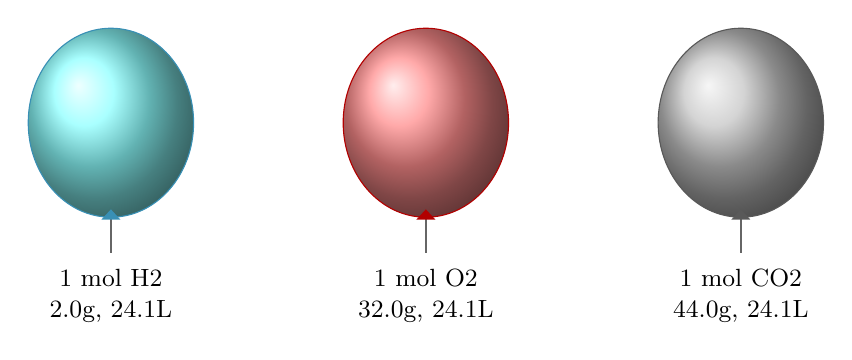
\begin{tikzpicture}[font=\small]
  \foreach \x/\g/\m/\c in {0/{\ce{H2}}/2.0/cyan, 4/{\ce{O2}}/32.0/red,
                           8/{\ce{CO2}}/44.0/gray} {
    \draw[thick, black!60] (\x,-0.25) -- (\x,-1.1);
    \shade[ball color=\c!45, draw=\c!70!black] (\x,0.55) ellipse (1.05 and 1.2);
    \fill[\c!70!black] (\x-0.12,-0.68) -- (\x+0.12,-0.68) -- (\x,-0.55) -- cycle;
    \node[align=center] at (\x,-1.65) {1 mol \g\\ \qty{\m}{g},
      \qty{24.1}{L}};
  }
\end{tikzpicture}

{\small Drie ballonnen bij \qty{20}{\celsius}, elk met één \omterm{def:g10:the-mole:amount}{mol} van een
ander gas. De volumes zijn gelijk; de massa's niet.}
\end{omfigure}


\begin{example}[Een ballon koolstofdioxide]\label{ex:g10:the-mole:balloon}
% ledger: aw:C, aw:O
Een ballon bevat \qty{2.4}{L} koolstofdioxide bij \qty{20}{\celsius}.
De hoeveelheid is $n = \qty{2.4}{L} / \qty{24.1}{L/mol} = \qty{0.10}{mol}$,
en de massa $m = \qty{0.10}{mol} \times \qty{44.0}{g/mol} =
\qty{4.4}{g}$. Dezelfde ballon gevuld met waterstof zou dezelfde
\qty{0.10}{mol} bevatten, maar maar \qty{0.20}{g} gas.
\end{example}

\begin{remark}[Zware en lichte gassen]\label{rem:g10:the-mole:heavy}
Omdat een liter van elk gas dezelfde hoeveelheid bevat, is de massa van
een liter gas evenredig met de \omterm{def:g10:the-mole:molar-mass}{molaire massa}. \omterm{def:g4:air-a-mixture-of-gases:air}{Lucht}, een \omterm{def:g6:pure-substances-and-mixtures:mixture}{mengsel} van
ongeveer vier vijfde stikstof (\qty{28.0}{g/mol}) en een vijfde zuurstof
(\qty{32.0}{g/mol}), gedraagt zich als een gas met een \omterm{def:g10:the-mole:molar-mass}{molaire massa} van
ongeveer \qty{29}{g/mol}. Een gas met een grotere \omterm{def:g10:the-mole:molar-mass}{molaire massa}, zoals
koolstofdioxide (\qty{44.0}{g/mol}), is dichter dan \omterm{def:g4:air-a-mixture-of-gases:air}{lucht} en verzamelt
zich onderin een gesloten kelder; een gas met een kleinere \omterm{def:g10:the-mole:molar-mass}{molaire massa},
zoals helium (\qty{4.0}{g/mol}), stijgt op.
\end{remark}

\section{Oefeningen}

\begin{exercise}[$\star$]\label{exo:g10:the-mole:1}
Bereken de \omterm{def:g10:the-mole:molar-mass}{molaire massa's} van zuurstof \ce{O2}, stikstof \ce{N2},
methaan \ce{CH4}, ammoniak \ce{NH3} en koolstofdioxide \ce{CO2}.
\end{exercise}

\begin{exercise}[$\star$]\label{exo:g10:the-mole:2}
Welke \omterm{def:g10:the-mole:amount}{hoeveelheid stof} zit er in \qty{36.0}{g} water? En in
\qty{4.0}{g} methaan?
\end{exercise}

\begin{exercise}[$\star$]\label{exo:g10:the-mole:3}
Wat is de massa van \qty{0.25}{mol} natriumchloride \ce{NaCl}? En van
\qty{2.0}{mol} koolstofdioxide?
\end{exercise}

\begin{exercise}[$\star$]\label{exo:g10:the-mole:4}
Hoeveel \omterm{def:g7:atoms-and-molecules:molecule}{moleculen} zitten er in \qty{0.50}{mol} zuurstof? Welke
hoeveelheid ijzer bevat \num{3.0e24} ijzeratomen?
\end{exercise}

\begin{exercise}[$\star$]\label{exo:g10:the-mole:5}
Welk volume neemt \qty{0.50}{mol} stikstof in bij \qty{20}{\celsius} en
normale atmosferische druk? Welke hoeveelheid zuurstof zit er in
\qty{12}{L} van dat gas?
\end{exercise}

\begin{exercise}[$\star\star$]\label{exo:g10:the-mole:6}
Een druppel water heeft een volume van \qty{0.050}{mL}, en \qty{1}{mL}
water heeft een massa van \qty{1.0}{g}. Hoeveel watermoleculen bevat de
druppel?
\end{exercise}

\begin{exercise}[$\star\star$]\label{exo:g10:the-mole:7}
Wat bevat meer \omterm{def:g7:atoms-and-molecules:atom}{atomen}, \qty{10}{g} aluminium of \qty{10}{g} ijzer? Leg
het eerst uit zonder te rekenen, en controleer het daarna met een
berekening.
\end{exercise}

\begin{exercise}[$\star\star$]\label{exo:g10:the-mole:8}
Bereken bij \qty{20}{\celsius} de massa van één liter koolstofdioxide en
van één liter stikstof. Waarom verzamelt koolstofdioxide zich onderin
een gesloten kelder waar druivensap gist?
\end{exercise}

\begin{exercise}[$\star\star$]\label{exo:g10:the-mole:9}
Geef met de figuur van de drie vakken $m$, $n$, $N$ de massa van
\num{1.0e22} \omterm{def:g7:atoms-and-molecules:molecule}{moleculen} glucose \ce{C6H12O6}. Schrijf de twee pijlen op
die je volgt.
\end{exercise}

\begin{exercise}[$\star\star$]\label{exo:g10:the-mole:10}
Een suikerklontje (sacharose, \ce{C12H22O11}) heeft een massa van
\qty{5.0}{g}. Bereken de hoeveelheid sacharose die het bevat, daarna het
aantal sacharosemoleculen, daarna het aantal koolstofatomen.
\end{exercise}

\begin{exercise}[$\star\star$]\label{exo:g10:the-mole:11}
Wat bevat de grootste hoeveelheid \omterm{def:g7:atoms-and-molecules:molecule}{moleculen}: \qty{1.0}{kg} water
\ce{H2O} of \qty{1.0}{kg} ethanol \ce{C2H6O}? Met welke factor?
\end{exercise}

\begin{exercise}[$\star\star\star$]\label{exo:g10:the-mole:12}
Een gouden ring heeft een massa van \qty{5.0}{g}; drie kwart van de massa
is goud, de rest koper. Hoeveel goudatomen bevat hij? Hoeveel
koperatomen? Van welk \omterm{def:g9:periodic-table-first-look:metal}{metaal} heeft de ring meer \omterm{def:g7:atoms-and-molecules:atom}{atomen}?
\end{exercise}

\begin{exercise}[$\star\star\star$]\label{exo:g10:the-mole:13}
Een lokaal is \qty{8.0}{m} bij \qty{6.0}{m} bij \qty{3.0}{m}, en de
\omterm{def:g4:air-a-mixture-of-gases:air}{lucht} erin heeft een temperatuur van \qty{20}{\celsius}.
\begin{enumerate}
  \item Welke hoeveelheid gas bevat het ($\qty{1}{m^3} =
        \qty{1000}{L}$)? Hoeveel \omterm{def:g7:atoms-and-molecules:molecule}{moleculen}?
  \item Neem voor \omterm{def:g4:air-a-mixture-of-gases:air}{lucht} op elke honderd \omterm{def:g7:atoms-and-molecules:molecule}{moleculen} 78 \omterm{def:g7:atoms-and-molecules:molecule}{moleculen} stikstof,
        21 zuurstof en 1 argon (\qty{40.0}{g/mol}), en bereken de
        gemiddelde \omterm{def:g10:the-mole:molar-mass}{molaire massa} van \omterm{def:g4:air-a-mixture-of-gases:air}{lucht}.
  \item Wat is de massa van de \omterm{def:g4:air-a-mixture-of-gases:air}{lucht} in het lokaal?
\end{enumerate}
\end{exercise}

\begin{exercise}[$\star\star\star$]\label{exo:g10:the-mole:14}
Een bol van zuiver silicium heeft een massa van precies \qty{1.000}{kg}.
\begin{enumerate}
  \item Hoeveel siliciumatomen bevat hij?
  \item Leid daaruit de massa van één siliciumatoom af.
  \item Vóór 2019 lag de \omterm{def:g10:the-mole:avogadro}{constante van Avogadro} niet vast, maar werd ze
        gemeten. Leg uit hoe een onafhankelijke telling van de \omterm{def:g7:atoms-and-molecules:atom}{atomen}
        van zo'n bol, waarvan de \omterm{def:g10:the-mole:amount}{hoeveelheid stof} bekend is uit de massa,
        een waarde voor die constante zou opleveren.
\end{enumerate}
\end{exercise}

\begin{exercise}[$\star\star\star$]\label{exo:g10:the-mole:15}
% ledger: iso:Cl35, iso:Cl37
Natuurlijk chloor bevat \qty{75.8}{\percent} \omterm{def:g7:atoms-and-molecules:atom}{atomen} chloor-35, met een
\omterm{def:g10:the-mole:molar-mass}{molaire massa} heel dicht bij \qty{35.0}{g/mol}, en \qty{24.2}{\percent}
\omterm{def:g7:atoms-and-molecules:atom}{atomen} chloor-37, met een \omterm{def:g10:the-mole:molar-mass}{molaire massa} heel dicht bij
\qty{37.0}{g/mol}. Bereken de \omterm{def:g10:the-mole:molar-mass}{molaire atoommassa} van natuurlijk chloor, en
vergelijk die met de waarde uit de tabel.
\end{exercise}

\section{Probleem: Het glas water van Kelvin}

\begin{problem}[{Weekendprobleem --- giet een glas water in zee, wacht tot
het door alle oceanen gemengd is, en vul opnieuw een glas: hoeveel van de
eerste moleculen komen terug?}]
\label{pb:g10:the-mole:1}
% ledger: ocean:volume, rho:water, const:NA, aw:H, aw:O
Een beroemd gedachte-experiment, vaak toegeschreven aan de natuurkundige
Lord Kelvin, gaat zo. Markeer elk \omterm{def:g7:atoms-and-molecules:molecule}{molecuul} in een glas water, giet het
glas in zee, en wacht tot de gemarkeerde \omterm{def:g7:atoms-and-molecules:molecule}{moleculen} zich gelijkmatig over
alle oceanen van de wereld verspreid hebben. Schep dan het glas opnieuw
vol, waar dan ook in zee. Brengt het gemarkeerde \omterm{def:g7:atoms-and-molecules:molecule}{moleculen} terug? Het
glas bevat \qty{250}{mL}, en \qty{1}{mL} water heeft een massa van
\qty{1.0}{g}. De oceanen bevatten ongeveer \qty{1.335e9}{km^3} water.
Behandel zeewater bij het tellen als zuiver water.

\medskip
\noindent\textbf{Deel I --- Water in een glas.}
\begin{enumerate}
  \item Bereken de \omterm{def:g10:the-mole:molar-mass}{molaire massa} van water.
  \item Wat is de massa van het water in het glas?
  \item Bereken de hoeveelheid watermoleculen in het glas.
  \item Welke hoeveelheid waterstofatomen bevat het glas? En
        zuurstofatomen?
\end{enumerate}

\medskip
\noindent\textbf{Deel II --- \omterm{def:g7:atoms-and-molecules:molecule}{Moleculen} in het glas.}
\begin{enumerate}[resume]
  \item Hoeveel watermoleculen bevat het glas?
  \item Bereken de massa van één watermolecuul, in gram.
  \item Controleer de antwoorden op 5 en 6 door ze met elkaar te
        vermenigvuldigen: wat moet het product zijn?
  \item Hoeveel jaar zou het duren om de \omterm{def:g7:atoms-and-molecules:molecule}{moleculen} van het glas te
        tellen, als je dag en nacht één \omterm{def:g7:atoms-and-molecules:molecule}{molecuul} per seconde telt? (Een
        jaar duurt ongeveer \qty{3.16e7}{s}.)
\end{enumerate}

\medskip
\noindent\textbf{Deel III --- De oceaan.}
\begin{enumerate}[resume]
  \item Reken het volume van de oceanen om naar kubieke meter
        ($\qty{1}{km^3} = \qty{e9}{m^3}$), en daarna naar liter.
  \item Hoeveel gemarkeerde \omterm{def:g7:atoms-and-molecules:molecule}{moleculen} zitten er in elke liter oceaan, als
        ze zich gelijkmatig verspreid hebben?
  \item Hoeveel gemarkeerde \omterm{def:g7:atoms-and-molecules:molecule}{moleculen} brengt het tweede glas terug?
  \item Tweede methode. Bereken de hoeveelheid water in de oceanen, met
        \qty{1.0}{kg} voor de massa van één liter.
  \item Welk deel van alle watermoleculen van de oceaan is gemarkeerd?
  \item Vermenigvuldig dit deel met het aantal \omterm{def:g7:atoms-and-molecules:molecule}{moleculen} van het tweede
        glas, en vergelijk met het antwoord op vraag 11.
\end{enumerate}

\medskip
\noindent\textbf{Deel IV --- Wat het betekent.}
\begin{enumerate}[resume]
  \item Hoeveel glazen van \qty{250}{mL} zou je met het water van de
        oceanen kunnen vullen?
  \item Vergelijk dit getal met het aantal \omterm{def:g7:atoms-and-molecules:molecule}{moleculen} van één glas. Leg in
        één zin uit waarom het tweede glas zoveel gemarkeerde \omterm{def:g7:atoms-and-molecules:molecule}{moleculen}
        terugbrengt.
  \item Hoeveel zeewater moet je gemiddeld scheppen om één enkel
        gemarkeerd \omterm{def:g7:atoms-and-molecules:molecule}{molecuul} terug te krijgen? Vergelijk met een druppel
        van \qty{0.05}{mL}.
  \item Het antwoord op vraag 11 heeft veel cijfers. Waarom zou je het
        alleen als orde van grootte moeten geven? Geef twee redenen.
  \item Geef het eindantwoord: ongeveer hoeveel \omterm{def:g7:atoms-and-molecules:molecule}{moleculen} van het eerste
        glas komen terug in het tweede?
\end{enumerate}
\end{problem}
